\begin{frame}{Kernel generation}
  \begin{columns}[c]
    \column{.54\textwidth}
    \only<1>{%
        \begin{block}{Hits}
        \begin{itemize}
            \item Hits lie on the 26 planes
            \item Tracks come from PVs and SVs
            \item For simplicity, only 3 tracks shown
            \item Hits are sorted in $r$ (distance from LHC beam)
        \end{itemize}
        \end{block}
    }
    \only<2>{%
        \begin{block}{Grid}
        \begin{itemize}
            \item Make a 3D grid of voxels (2D shown)
            \item \textcolor{lhcbRed}{Note: only $z$ will be fully calculated and stored}
        \end{itemize}
        \end{block}
    }
    \only<3-5>{%
        \begin{block}{Prototrack}
        \begin{itemize}
            \item Start with sorted $r$
            \item Find triplet with $\chi^2<10$
            \item Mark ``used'' all other hits within $\chi^2<9$
            \item \textcolor{lhcbRed}{Note: triplet is stored}
        \end{itemize}
        \end{block}

        \begin{block}{Kernel}
        \begin{itemize}
            \item Fill in each voxel center with gaussian PDF
            \item PDF is combined for each prototrack
        \end{itemize}
        \end{block}

    }
    \only<6>{%
        \begin{block}{Kernel}
        \begin{itemize}
            \item Highest PDF density at vertices
            \item Stores $z$ histogram with maximum PDF values
        \end{itemize}
        \end{block}

        \begin{block}{Details}
        \begin{itemize} \color{lhcbRed}
            \item $x$-$y$ grid initially very coarse
            \item Search performed on maximum $x$-$y$ grid cell using stored triplets to recalculate PDF
        \end{itemize}
        \end{block}
    }

    \column{.46\textwidth}
    \begin{tikzpicture}
        [hit/.style={inner sep=2pt, fill, circle, black!80!red},
        simitrack/.style={shorten >= -6cm, shorten <= -6cm, opacity=.2, line width=.1cm,
            preaction={draw, line width=.3cm, opacity=.2},
            preaction={draw, line width=.5cm, opacity=.2}},
        bluesimitrack/.style={thick, blue,
            preaction={shorten >= -6cm, shorten <= -6cm, draw, opacity=.2, line width=.1cm,
                preaction={draw, blue, line width=.3cm, opacity=.2},
                preaction={draw, blue, line width=.5cm, opacity=.2}}}
        ]

        \node at (2,-3) [below] {$z$ axis (along the beam)};
        \node at (-1, 0) [left] {$x$};

        \clip (-1,-3) rectangle (5,3);

        \begin{scope}[xscale=.65, xshift=-.6cm]

        % def f(name, slope, factor):
        %     v = np.arange(1,9)
        %     vv = (v-.5)*slope + .05*np.sin(v*factor)
        %     q = np.linspace(.5, 8, 400)
        %     qq = (q-.5)*slope + .05*np.sin(q*factor)
        %     print(f'% {name} slope={slope} factor={factor}')
        %     for a,b in zip(v,vv):
        %         print(f'\coordinate ({name}{a}) at ({a}, {b:.3});')
        %     print()
        %     return q, qq, v, vv


        % (v-.5)*slope + .05*np.sin(v*factor)
        % A slope=0.4 factor=-5
        \coordinate (A7) at (1, 0.248);
        \coordinate (A6) at (2, 0.627);
        \coordinate (A5) at (3, 0.967);
        \coordinate (A4) at (4, 1.35);
        \coordinate (A3) at (5, 1.81);
        \coordinate (A2) at (6, 2.25);
        \coordinate (A1) at (7, 2.62);

        % B slope=0.06 factor=6
        \coordinate (B8) at (1, 0.016);
        \coordinate (B7) at (2, 0.0632);
        \coordinate (B6) at (3, 0.112);
        \coordinate (B5) at (4, 0.165);
        \coordinate (B4) at (5, 0.221);
        \coordinate (B3) at (6, 0.28);
        \coordinate (B2) at (7, 0.344);
        \coordinate (B1) at (8, 0.412);

        % C slope=-0.35 factor=7
        \coordinate (C7) at (1, -0.142);
        \coordinate (C6) at (2, -0.475);
        \coordinate (C5) at (3, -0.833);
        \coordinate (C4) at (4, -1.21);
        \coordinate (C3) at (5, -1.6);
        \coordinate (C2) at (6, -1.97);
        \coordinate (C1) at (7, -2.32);

        \only<1>{%
        \foreach \x in {0,...,9}{%
            \draw [ultra thick, yellow!80!black] (\x, -3) -- (\x,3);
        }
        }
        \end{scope}

        \only<2->{%
        \draw[step=.5, gray, very thin, use as bounding box] (-1,-3) grid (5,3);
        }

        \only<3>{%
            \draw [bluesimitrack] (A5) -- (A7) ;
        } \only<4->{%
            \draw [simitrack] (A5) -- (A7) ;
        }

        \only<4>{%
            \draw [bluesimitrack] (B6) -- (B8) ;
        } \only<5->{%
            \draw [simitrack] (B6) -- (B8) ;
        }

        \only<5>{%
            \draw [bluesimitrack] (C5) -- (C7) ;
        } \only<6->{%
            \draw [simitrack] (C5) -- (C7) ;
        }

        \draw [fill,green!60!black] (0,0) circle (.065) node [left] {PV};

        \only<0-2>{%
        \node [hit] at (A1) {};
        \node [hit] at (A2) {};
        \node [hit] at (A3) {};
        \node [hit] at (A4) {};
        }\only<3->{%
        \node [hit, red] at (A1) {};
        \node [hit, red] at (A2) {};
        \node [hit, red] at (A3) {};
        \node [hit, red] at (A4) {};
        }

        \only<0-2>{%
        \node [hit] at (A5) {};
        \node [hit] at (A6) {};
        \node [hit] at (A7) {};
        } \only<3>{%
        \node [hit, blue] at (A5) {};
        \node [hit, blue] at (A6) {};
        \node [hit, blue] at (A7) {};
        } \only<4->{%
        \node [hit, red] at (A5) {};
        \node [hit, red] at (A6) {};
        \node [hit, red] at (A7) {};
        }

        \only<0-3>{%
        \node [hit] at (B1) {};
        \node [hit] at (B2) {};
        \node [hit] at (B3) {};
        \node [hit] at (B4) {};
        \node [hit] at (B5) {};
        } \only<4->{%
        \node [hit, red] at (B1) {};
        \node [hit, red] at (B2) {};
        \node [hit, red] at (B3) {};
        \node [hit, red] at (B4) {};
        \node [hit, red] at (B5) {};
        }

        \only<0-3>{%
        \node [hit] at (B6) {};
        \node [hit] at (B7) {};
        \node [hit] at (B8) {};
        } \only<4>{%
        \node [hit, blue] at (B6) {};
        \node [hit, blue] at (B7) {};
        \node [hit, blue] at (B8) {};
        }\only<5->{%
        \node [hit, red] at (B6) {};
        \node [hit, red] at (B7) {};
        \node [hit, red] at (B8) {};
        }

        \only<0-4>{%
        \node [hit] at (C1) {};
        \node [hit] at (C2) {};
        \node [hit] at (C3) {};
        \node [hit] at (C4) {};
        } \only<5->{%
        \node [hit, red] at (C1) {};
        \node [hit, red] at (C2) {};
        \node [hit, red] at (C3) {};
        \node [hit, red] at (C4) {};
        }

        \only<0-4>{%
        \node [hit] at (C5) {};
        \node [hit] at (C6) {};
        \node [hit] at (C7) {};
        } \only<5>{%
        \node [hit, blue] at (C5) {};
        \node [hit, blue] at (C6) {};
        \node [hit, blue] at (C7) {};
        } \only<6->{%
        \node [hit, red] at (C5) {};
        \node [hit, red] at (C6) {};
        \node [hit, red] at (C7) {};
        }

    \end{tikzpicture}

    \end{columns}
\end{frame}
